\clearpage
\chapter{Design \& Implementation}

Now that the fundamental mathematics of numerical technique has been covered, in this chapter, the general approach to implementing the finite element method in serial is discussed. The design structure of the code is explained, such as data structures and classes used, and storage approaches such as the benefits of applying sparse storage formats and sparse solvers. The use of linear algebra libraries, specifically Intel's MKL, are detailed as they were utilised to avoid reinventing the wheel when solving the final linear system. 

\section{General Approach}

Given that there is a lot of machinery involved in programming the FEM as a numerical method, steps were taken to break the code up into as many logical partitions as possible and structure it in a such a way which made sense from a glance. All the serial code was written in C++11, allowing use of object oriented programming and many of the newer features of the standard library (STL) such as auto types and ordered sets. A large benefit here also was the inbuilt RAII features of C++, reducing the need for manual memory management - important here when it will become clear there is much memory to be allocated to code a FEM implementation.

\subsection{Design Structure}
\begin{figure}
	\centering
	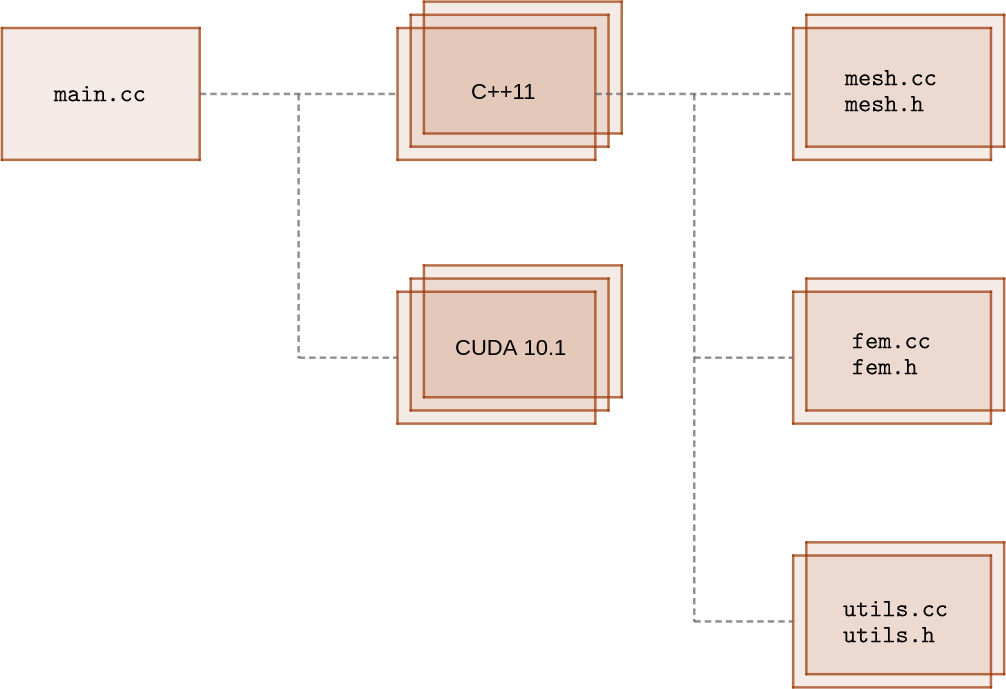
\includegraphics[width = 0.7\linewidth]{Figures/cpp_code}
	\caption{Code structure of the C++ code implementation.}
	\label{fig:cpp}
\end{figure}

Figure~\ref{fig:cpp} illustrates the overall design structure of the code - in both serial and parallel, though the GPU code will be discussed in more detail in Section~\ref{gpucode}. The code is split into four main files and their respective headers,
\begin{itemize}
	\item \texttt{main.cc} - Main C++ code, used for invoking the FEM operation and calling results to be output.
	\item \texttt{mesh.cc} - Contains the code for the Mesh class, storing all necessary operations and data structures to construct a mesh.
	\item \texttt{fem.cc} - Code for a FEM class which contains the routines needed to perform the method on a given mesh.
	\item \texttt{utils.cc} - General utility functions, such as SSE, parsing of command line arguments et cetera.
\end{itemize}
The approach here would be that a Mesh object be created, passed to a FEM object as an input parameter to a constructor, the FEM would complete the routine and the utility functions would perform sundry operations after this to tidy up. Figure~\ref{fig:serial_flow} demonstrates a flowchart of the serial code process.
\begin{figure}
	\centering
	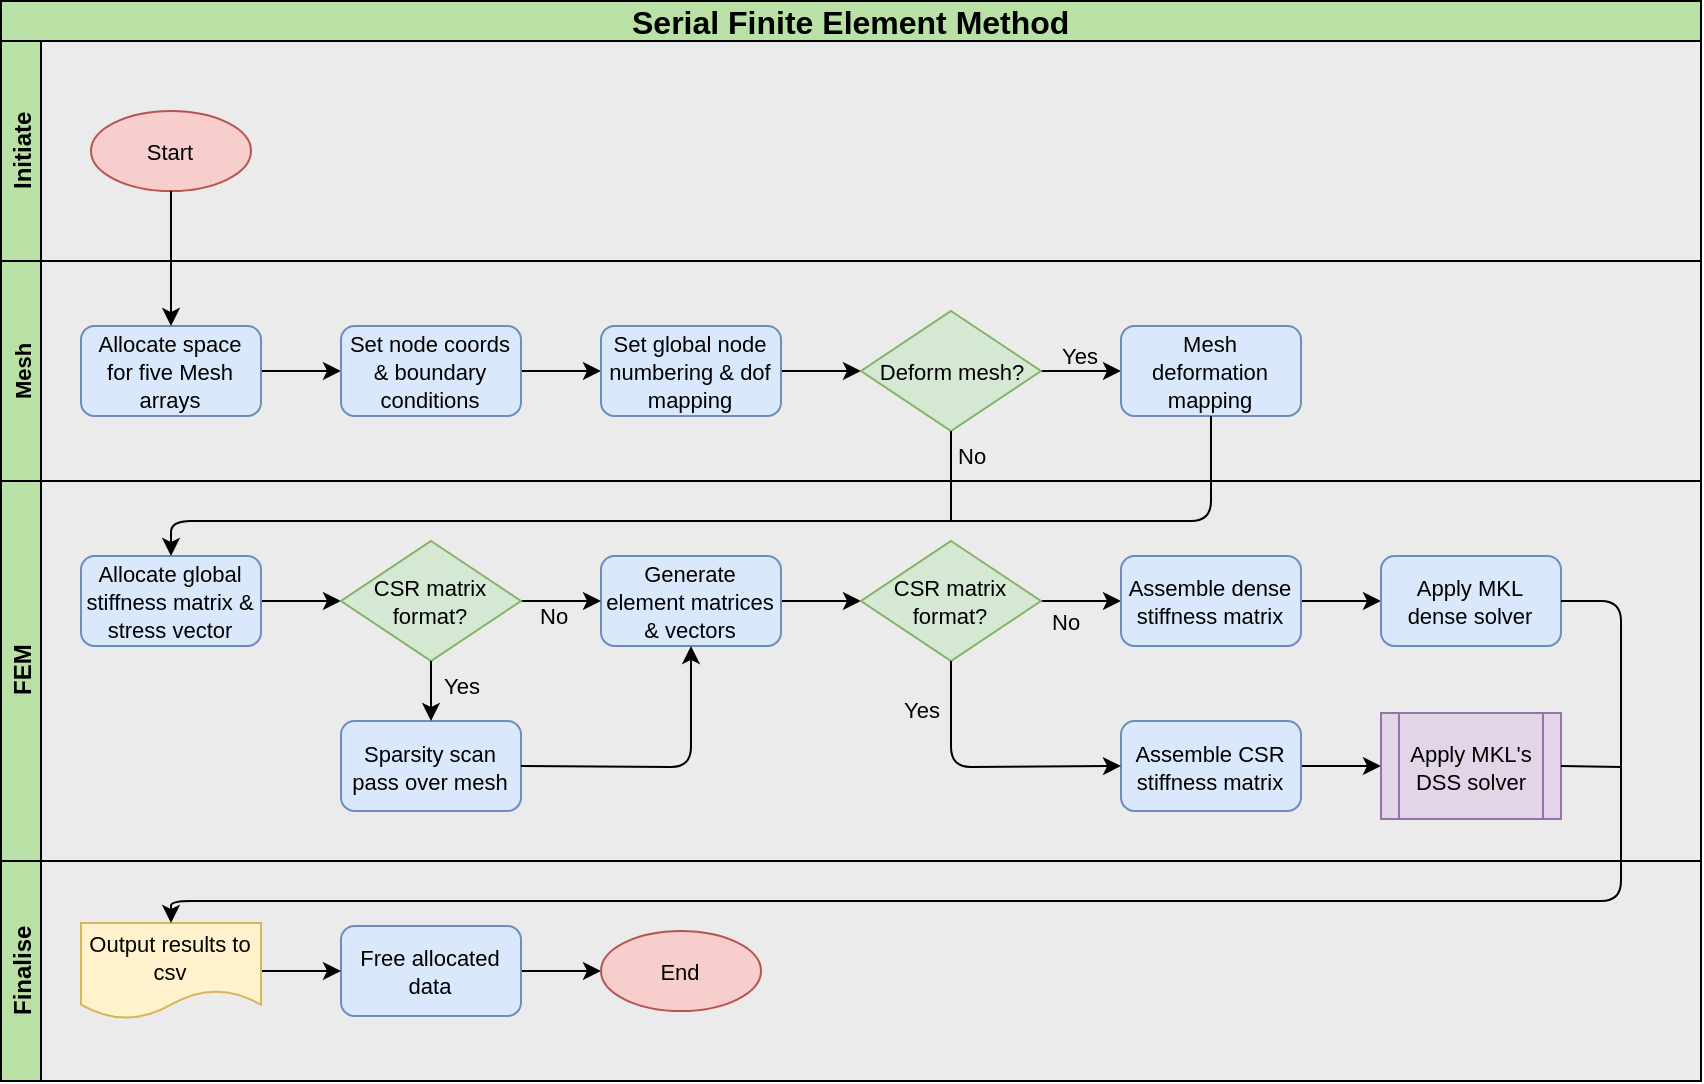
\includegraphics[width = 0.9\linewidth]{Figures/serial_flowchart}
	\caption{Flowchart of serial FEM implementation.}
	\label{fig:serial_flow}
\end{figure}

\section{Data Structures}

Objects are a massive sell for using C++ over C when programming a numerical method, for reasons stated already. For this paper, two classes were written, one to handle the mesh creation and one to handle performing FEM. In terms of other data structures, there was also a struct \texttt{Tau} to manage timings of all the operations without needing to pass around multiple variables in as function parameters.

\subsection{Mesh}\label{mesh}

The mathematics of the mesh has been illustrated, the next logical step would be to port it over to code. The data structure for the mesh holds a handful of key components and routines needed for its generation. Given the mesh itself is of course, a collection of interconnected nodes on a plane, upon each of which numerical calculations must be performed, it was naturally necessary to stores these nodes and their corresponding coordinates. In the implementation of this paper, a 2D mesh was used, though the extension to higher dimensions is rather arbitrary - another benefit of the FEM. The nodes' coordinates were stored in an array, \texttt{vertices}, which had a dimension of \texttt{order}, where order is the number of nodes or number of unknowns. Looking back at the Section~\ref{elems}, however, simply knowing the nodes coordinates for the FEM isn't enough, one also needs to know their global indices and degree of freedom mapping back to the stiffness matrix. These were respectively stored in two 2D arrays, \texttt{cells} and \texttt{dof}. Note that this is the exact same as performing the mapping function $q(e,r)$ seen previously. For example, \texttt{dof[e][r]} will provide the global node index of local node $r$ in cell $e$. Figure (REFERENCE) gives an example of a small mesh, the populated version of these three arrays are described in (LISTING). Note also in this example that each cell's array is numbered in an anti-clockwise direction - this is important for the orientation of the integrals calculated later. Since in this paper, only P1 examples were used, the degree of freedom mapping and global node indices are actually equal and so having two separate arrays for these was rather unnecessary but it allows for potential further expansion of the code with ease.

\begin{remark}
	Standard library vectors were not used for the 2D arrays as the contiguity of the data was important for transferring the data to the GPU and for certain linear solvers.
\end{remark}

In terms of what routines are contained in the Mesh class, during instantiation, the constructor creates a generic, rectangular mesh and populates the three arrays. There is a routine, whereby one can pass a mapping function as a parameter and deform the mesh. The aim of the deformation function is simply the fact that most FEM meshes aren't standard rectangles, apart from this particular test case - since the focus here is on a GPU optimisation. Other routines in the class then are merely to return various properties of the object: coordinates, pointers to the arrays (for CUDA purposes), number of nodes et cetera. There is also a routine to do a pass over the mesh and return its sparsity pattern which is detailed in Section~\ref{sparsity}.

\subsection{FEM}

Once the mesh has been generated, the next aim for the software was to create as generic a FEM class as possible, one which could take any mesh in the structure of the Mesh class, and solve the given PDE - in this report's case the Laplace equation. The FEM class will, of course, need to allocate data to store the global stiffness matrix and global stress vectors. The stress vector is simply stored in \texttt{b} and has a dimension of \texttt{order}, the stiffness matrix on the other hand can be stored in either dense or CSR format. Since CSR is stored in three separate, single dimensional arrays, this allowed the benefit of using standard library vectors, also eliminating the need for \texttt{new} and \texttt{delete}. The dense format on the other hand is 2D and has the same issue with contiguity as mentioned in the remark above. The CSR matrix is stored in \texttt{valsL}, \texttt{rowPtrL} and \texttt{colIndL} and the dense matrix is stored in \texttt{L}. The class then also stores certain properties needed, such as the dimensions of the problem \texttt{order}, the number of cells in the mesh and the number of non-zeros in the sparse matrix.

From a routine perspective, this is where all the real nuts and bolts of the FEM come into play.  There are three primary routines here which need to be completed in order to obtain a solution:
\begin{enumerate}
	\item element matrix generation.
	\item global stiffness matrix and stress vector assembly.
	\item linear system solver.
\end{enumerate}
The element matrix calculation is detailed in Algorithm (REFERENCE), utilising the convenient formulas stated in Section~\ref{problem}. The assembly routine on the other hand, has two different variants, one to handle the dense matrix assembly and one to handle assembling in CSR. Algorithms (REFRENCEx2) show both variants of this assembly. The last main routine, solving the linear system was handled by Intel's MKL library, taking advantage of pre-existing, optimised kernels.

\section{Sparse Storage}\label{sparse}

\begin{figure}
	\centering
	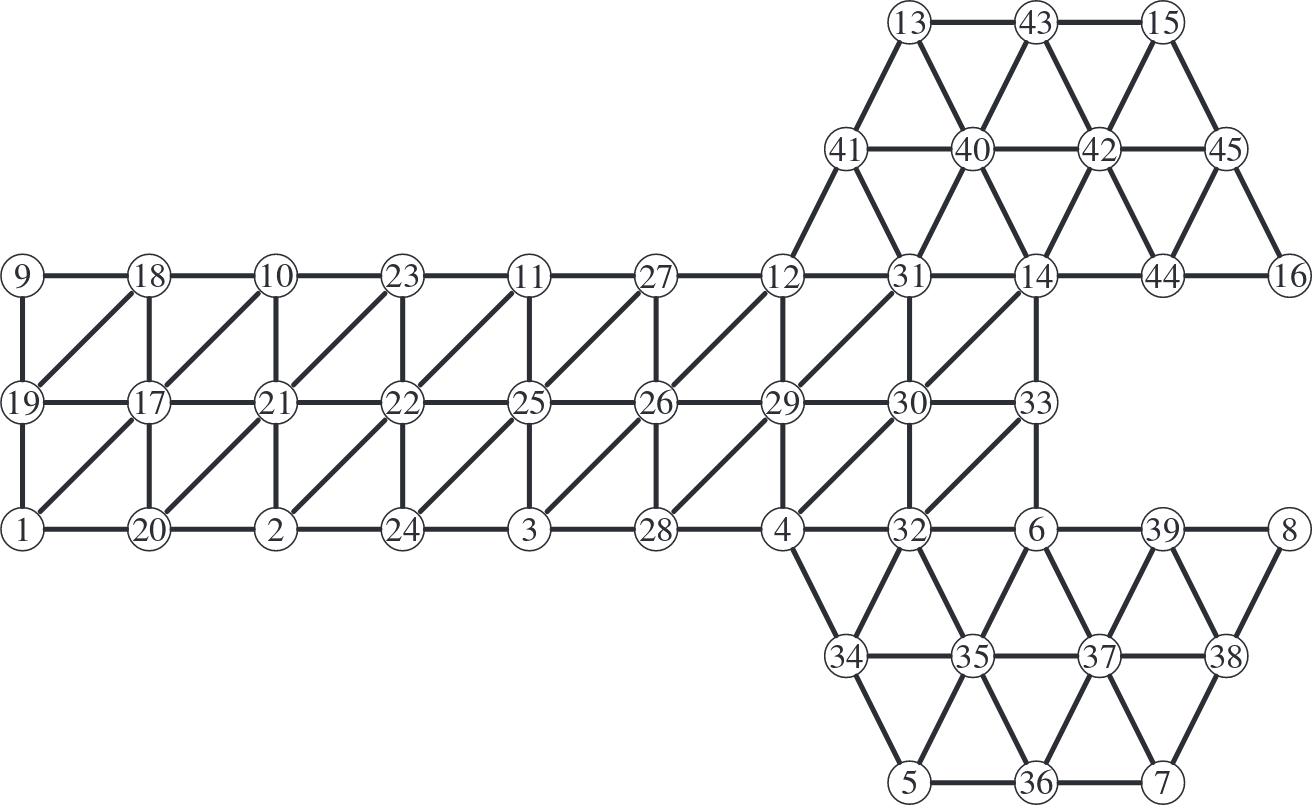
\includegraphics[width=0.7\linewidth]{Figures/mesh_graph}
	\caption{Mesh for generic FEM problem illustrated as a graph representation.}
	\label{fig:graph}
\end{figure}
\begin{figure}
	\centering
	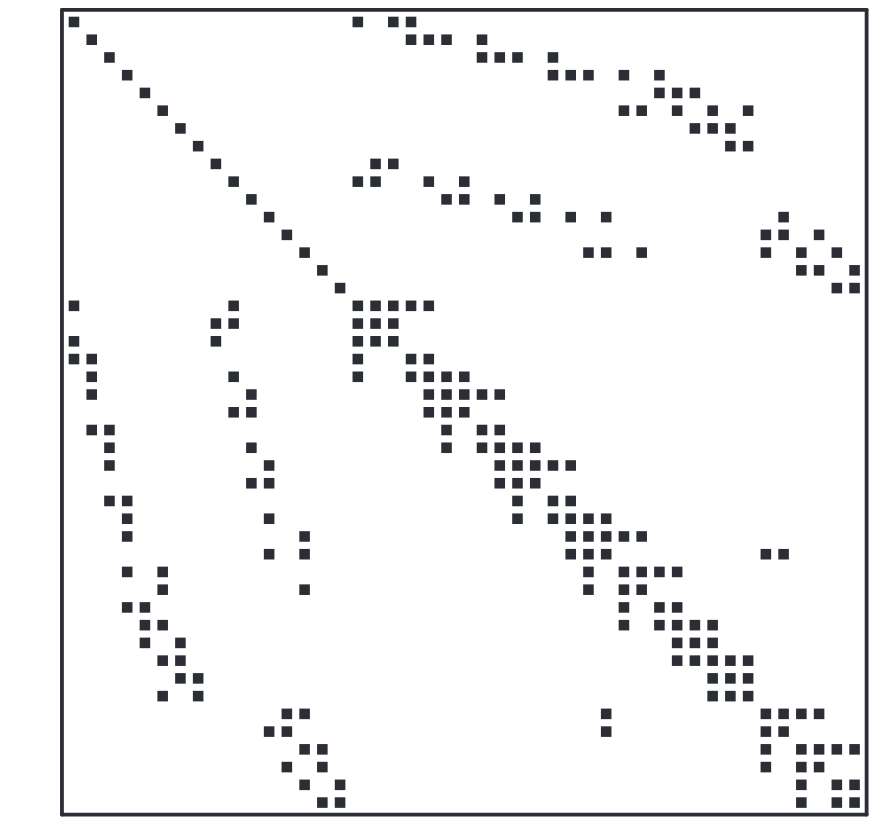
\includegraphics[width=0.4\linewidth]{Figures/sparsity_pattern}
	\caption{Sparsity pattern of FEM mesh.}
	\label{fig:pattern}
\end{figure}

The idea of sparse matrices and CSR storage has been thrown about in this paper a handful of times. The idea here is that a matrix is considered sparse, if if consists of mostly 0 valued entries - in some papers it is defined as having over 50\% 0 entries but this is a rather loose definition. This is important in the FEM as, if the basis functions are considered, one must remember that these are defined on a compact support $\Omega^{(e)}$, and will be 0 everywhere outside of this domain. Due to this, the global stiffness matrix will be a SPD, sparse matrix. Consider again Figure (REFERENCE), at no point is there any connection between nodes X and Y, thus the resulting inner product $\left\langle\varphi_X,\varphi_Y\right\rangle=0$. Why is this important? It can be hugely beneficial to computation time if one can take advantage of the sparsity pattern of a matrix, clearly as there is going to be potentially orders less null operations to iterate through.

These matrices can be stored in a number of different ways, three will be looked at here, although only CSR was used in the implementation:
\begin{itemize}
	\item CSR.
	\item CSC.
	\item COO.
\end{itemize}
CSR or \textit{compressed sparse row} storage is the most commonly used variant of sparse storage. As mentioned, it works by storing the matrix into three separate arrays, $A$, containing all the non-zero values, $IA$, the indices of the beginning of each row in the array $A$ and has a length of $n+1$ where $n$ is the number or rows, and finally $JA$, the indices of the column each value in $A$ is in. For more clarity, consider the matrix,
\begin{equation}
	A = 
	\left[\begin{matrix}
		3 & 1 & 0 & 0 & 0\\
		0 & 20 & 15 & 0 & 1\\
		0 & 0 & 0 & 4 & 1\\
		9 & 1 & 6 & 8 & 0\\
		0 & 0 & 0 & 7 & 0\\
		0 & 0 & 0 & 0 & 11
	\end{matrix}\right],
\end{equation}
in CSR format this can be written as,
\begin{lstlisting}
 A = [ 3 1 20 15 1 4 1 9 1 6 8 7 11 ]
IA = [ 0 2 5 7 11 12 13 ]
IJ = [ 0 1 1 2 4 3 4 0 1 2 3 3 4 ]
\end{lstlisting}
In the case of this implementation, \texttt{valsL} = A, \texttt{rowPtrL} = AI and \texttt{colIndL} = IJ. An important thing to note is that these can be either 0-based indexing or 1-based indexing. Since this report didn't utilise any FORTRAN code, 0-based indexing was used in all cases.

\textit{Compressed sparse column} is almost identical to CSR storage, except it is column-major format instead. The same example matrix in CSC would give,
\begin{lstlisting}
 A = [ 3 9 1 20 1 15 6 4 8 7 1 1 11 ]
IA = [ 0 3 0 1 3 1 3 2 3 4 1 2 5 ]
IJ = [ 0 2 5 7 10 13 ].
\end{lstlisting}
Clearly here, IJ has dimensions $m+1$, where $m$ is the number of columns.

The last commonly used sparse storage format is \textit{coordinate lists} or COO, which stores the values and their coordinates in both row and column. Keeping with the same example gives,
\begin{lstlisting}
 A = [ 3 1 20 15 1 4 1 9 1 6 8 7 11 ]
IA = [ 0 0 1 1 1 2 2 3 3 3 3 4 5 ]
IJ = [ 0 1 1 2 4 3 4 0 1 2 3 3 4 ].
\end{lstlisting}
This can of course be done in either row-major or column-major directions.

\subsection{Graph Theory}

Looking at the sparsity of a matrix, this can be equated to graph traversal problems in graph theory. If we consider a graph problem $G(V,E)$, defined as a set of vertices,
\begin{equation}
	V = \{v_0,v_1,\dots,v_n\},
\end{equation}
and a set of edges $E$, consisting of pairs of vertices $v_i,v_j$, such that,
\begin{equation}
	E \subseteq V\times V.
\end{equation}
From a sparse matrix perspective, this graph can be thought of as the connectivity between elements in the matrix, i.e. if $\{v_i,v_j\} \in E$, then it can be shown that for a sparse matrix $A$, $A_{i,j}$ is non-zero. Looking at Figure~\ref{fig:graph}, demonstrating a mesh for a FEM problem in the form of a graph. Clearly all the edges and connectivity are clear from the figure, but this also gives us the inherent sparsity patter in the resulting matrix. Figure~\ref{fig:pattern} demonstrates this resulting global stiffness matrix. Thinking back to how the FEM, particularly its elements were defined, this result makes sense. The basis functions were defined on a compact support of touching nodes, so clearly if $\{v_i,v_j\} \notin E$, then the resulting inner-product,
\begin{equation}
	\left\langle \varphi_i, \varphi_j \right\rangle = 0.
\end{equation}

\subsection{Sparsity Scan}\label{sparsity}

Naturally, the next question needing to be posed is, how does one take advantage of this inherent sparsity pattern available in the stiffness matrix. The easiest, although there have been papers published on more advanced methods (CITE), is to run a single pass over the mesh to begin, taking the computational hit, and using this to create a sparsity pattern. In this implementation, the pass created a vector of STL sets, one set for each node, and iterated through each, amending to the set if there was an edge between the two nodes. Using this, one now has the number of non-zeros and can populate quite easily, IA and IJ, in the CSR matrix. Algorithm (REFERENCE) details how this is explicitly performed.

\section{Solver Libraries}

A substantial part of the computation time in the FEM, relies on actually solving the final linear system. While this report is aimed at optimising the FEM in general, it does not aim at optimising linear solvers - something which has been covered by countless PhD students and doctors over many years. Instead, a decision was made to simply use a pre-existing library for both convenience and efficiency's sake. There are many variants that could have been used, GNU Standard Library, MAGMA, LAPACK etc. The one which was used in the end was Intel's MKL.

\subsection{Intel's MKL}\label{mkl}

The Intel library was split into two separate sub-libraries: their LAPACK routines for dense systems, and their Direct Sparse Solver (DSS). Both were used in this paper for comparison reasons. In either case, given that the stiffness matrix $A$, is symmetric positive definite (SPD), both dense and sparse solvers work by initially factorising the matrix using Cholesky decomposition, $A = L^T L$, where $L$ is lower-triangular. This new system is now solved using a direct solver. The DSS also has an option of providing a reordering of the sparse matrix, prior to the Cholesky decomposition, such as Cuthill-McKee (CITE), if one so wishes to make the sparsity pattern more compact, and thus more efficient for solving. Figure~\ref{fig:ordering} demonstrates the potential benefits of reordering, a much more compact data set, allowing for far more coalesced operations and less distance to travel along memory (CITE MATLAB SITE). This option was left on "auto" for the purposes of this report. 
CITE INTEL'S DOCUMENTATION
\begin{figure}
    \centering
    \begin{subfigure}{0.49\textwidth}
        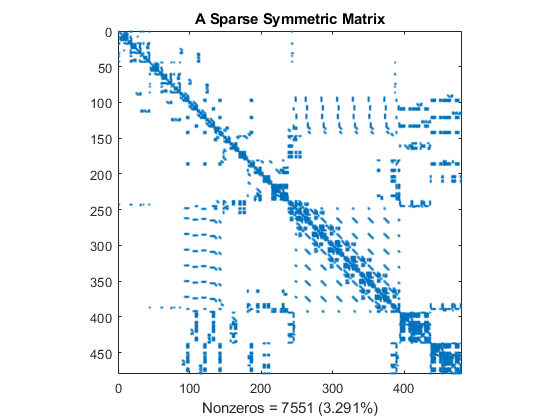
\includegraphics[width=\textwidth]{Figures/sparsity_unordered}
    \end{subfigure} \hfill
    \begin{subfigure}{0.49\textwidth}
        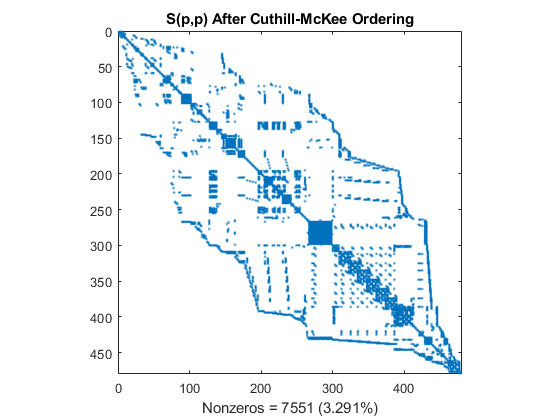
\includegraphics[width=\textwidth]{Figures/sparsity_cmckee}
    \end{subfigure} \\
    \begin{subfigure}{0.49\textwidth}
        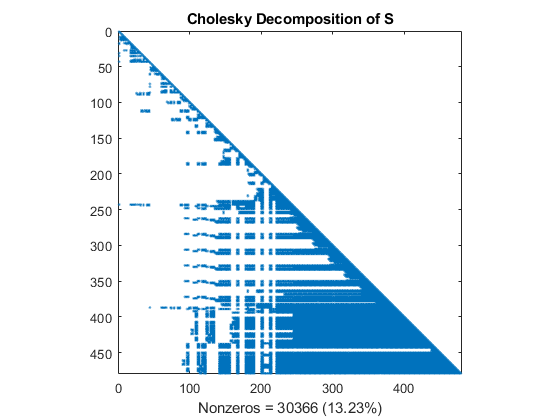
\includegraphics[width=\textwidth]{Figures/chol_unordered}
    \end{subfigure}\hfill
     \begin{subfigure}{0.49\textwidth}
        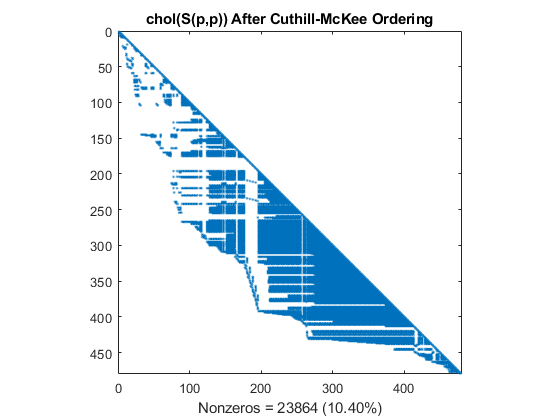
\includegraphics[width=\textwidth]{Figures/chol_cmckee}
    \end{subfigure}
    \caption{Illustration of a sparsity pattern of a matrix, pre and post Cuthill-McKee reordering, allong with the resulting Cholesky decompositions of both matrices.}
    \label{fig:ordering}
\end{figure}